\documentclass[10pt]{beamer}
\usetheme{metropolis}
\usepackage[utf8]{inputenc}
\usepackage[T1]{fontenc}
\usepackage{bookmark}
\usepackage{tikz}
\usetikzlibrary{shapes.geometric, arrows, positioning, shadows, calc}
\usepackage{listings}
\usepackage{xcolor}

% Custom Colors
\definecolor{DeepNavy}{HTML}{011627}
\definecolor{Slate}{HTML}{2E3440}
\definecolor{Emerald}{HTML}{2ECC71}
\definecolor{N8NBlue}{HTML}{FF6D5A} % N8N accent color

\setbeamercolor{palette primary}{bg=DeepNavy, fg=white}
\setbeamercolor{background canvas}{bg=white}

\title{Autonomous Research Agent (ARA)}
\subtitle{Orchestrating AI for Q1-Grade Literature Reviews}
\author{Bilel Ammouri}
\institute{Advanced Agentic Coding -- Research Division}
\date{\today}

\begin{document}

% --- Slide 1: Title ---
\begin{frame}
    \titlepage
\end{frame}

% --- Slide 2: Table of Contents ---
%\begin{frame}{Plan of the Presentation}
   % \tableofcontents
%\end{frame}

% --- Slide 3: The Vision ---
\section{Vision \& Problem}
\begin{frame}{The Vision of ARA}
    \begin{itemize}
        \item \textbf{Autonomous Mastery}: Transform a simple research theme into a 30-page academic manuscript.
        \item \textbf{High-Impact Focused}: Targeting Q1 journal standards through rigorous bibliometric analysis.
        \item \textbf{Agentic Intelligence}: Moving beyond templates to dynamic, self-planning synthesis.
    \end{itemize}
    \vfill
    \begin{exampleblock}{The Goal}
        Bridging the gap between raw web data and structured, peer-reviewable academic knowledge.
    \end{exampleblock}
\end{frame}

% --- Slide 4: The Core Problem ---
\begin{frame}{The Problem: Information Overload}
    \begin{columns}
        \begin{column}{0.5\textwidth}
            \begin{itemize}
                \item 5M+ papers published annually.
                \item "Hallucination" risks in standard LLMs.
                \item Disconnected data: Bibliometry vs. Synthesis.
            \end{itemize}
        \end{column}
        \begin{column}{0.5\textwidth}
            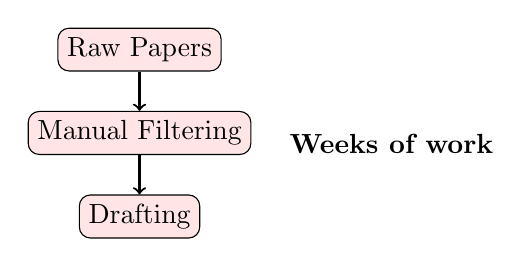
\begin{tikzpicture}[scale=0.8]
                \node (p1) [draw, fill=red!10, rounded corners] {Raw Papers};
                \node (p2) [below=0.5cm of p1, draw, fill=red!10, rounded corners] {Manual Filtering};
                \node (p3) [below=0.5cm of p2, draw, fill=red!10, rounded corners] {Drafting};
                \draw[->, thick] (p1) -- (p2);
                \draw[->, thick] (p2) -- (p3);
                \node at (4,-1.5) {\textbf{Weeks of work}};
            \end{tikzpicture}
        \end{column}
    \end{columns}
\end{frame}

% --- Slide 5: N8N Workflow (Global View) ---
\section{Global Workflow}
\begin{frame}{Global Workflow Orchestration}
    \centering
    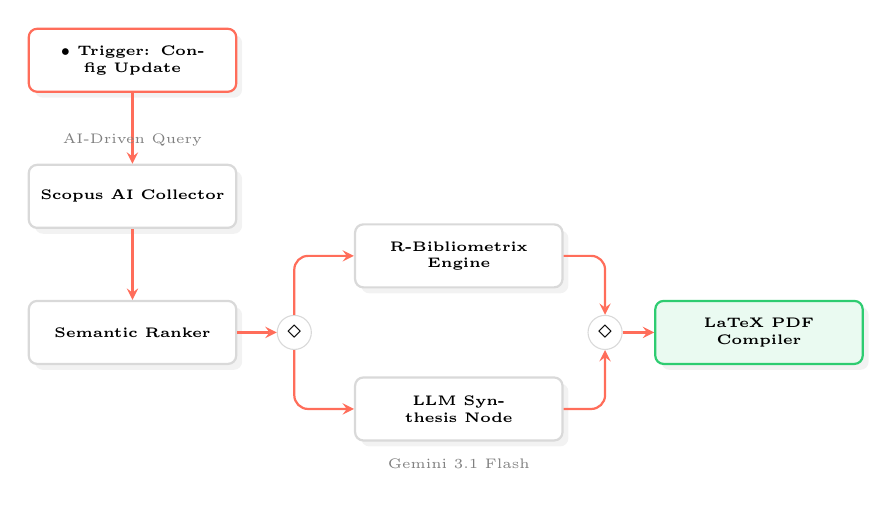
\begin{tikzpicture}[
        node distance=0.5cm and 0.8cm,
        n8nnode/.style={rectangle, draw=gray!30, fill=white, text width=2.4cm, text centered, rounded corners=3pt, minimum height=0.8cm, font=\tiny\bfseries, drop shadow={opacity=0.1}, thick},
        port/.style={circle, fill=gray!40, minimum size=3pt, inner sep=0pt},
        connector/.style={draw=N8NBlue, -stealth, thick, rounded corners=5pt}
    ]
        % Nodes
        \node (trigger) [n8nnode, draw=N8NBlue] {$\bullet$ Trigger: Config Update};
        \node (collector) [n8nnode, below=0.9cm of trigger] {Scopus AI Collector}; %right
        \node (ranker) [n8nnode, below=0.9cm of collector] {Semantic Ranker};
        \node (split) [circle, draw=gray!30, right=0.5cm of ranker, inner sep=2pt] {$\diamond$};
        
        \node (r_engine) [n8nnode, above right=0.4cm and 0.6cm of split] {R-Bibliometrix Engine};
        \node (llm_drafter) [n8nnode, below right=0.4cm and 0.6cm of split] {LLM Synthesis Node};
        
        \node (merge) [circle, draw=gray!30, right=3.5cm of split, inner sep=2pt] {$\diamond$};
        \node (output) [n8nnode, right=0.4cm of merge, fill=Emerald!10, draw=Emerald] {LaTeX PDF Compiler};

        % Connectors
        \draw [connector] (trigger) -- (collector);
        \draw [connector] (collector) -- (ranker);
        \draw [connector] (ranker) -- (split);
        \draw [connector] (split) |- (r_engine);
        \draw [connector] (split) |- (llm_drafter);
        \draw [connector] (r_engine) -| (merge);
        \draw [connector] (llm_drafter) -| (merge);
        \draw [connector] (merge) -- (output);
        
        % Labels
        \node [above=0.1cm of collector, font=\tiny, color=gray] {AI-Driven Query};
        \node [below=0.1cm of llm_drafter, font=\tiny, color=gray] {Gemini 3.1 Flash};
    \end{tikzpicture}
    \vfill
    \begin{tiny}
        A modular execution graph where each node represents a specific agentic responsibility.
    \end{tiny}
\end{frame}

% --- Slide 6: Brainstorming Workflow ---
\begin{frame}{Brainstorming: Why a Modular Workflow?}
    \begin{alertblock}{Design Strategy}
        We use a \textbf{Pipeline} pattern rather than a single LLM call.
    \end{alertblock}
    \vfill
    \begin{description}
        \item[Decoupling]: If Scopus API changes, only one module needs repair.
        \item[Groundedness]: The LLM "Drafter" only uses papers "Ranked" by the system—Zero Hallucination.
        \item[Diversity]: Combining Python (data), R (stats), and LaTeX (design).
    \end{description}
\end{frame}

% --- Slide 7: Functional Nodes - Collector ---
\section{Functional Deep Dive}
\begin{frame}{Node 1: Intelligent Scopus Collector}
    \textbf{Functionality}: Real-time academic retrieval.
    \vfill
    \begin{itemize}
        \item \textbf{AI Query Engine}: No more hardcoded keywords. Uses Gemini to generate optimized Boolean queries.
        \item \textbf{Metadata Enrichment}: Extracts `AU`, `TI`, `DE`, `C1`, `TC` and `AB` tags.
        \item \textbf{Resilience}: Handles "404 Not Found" and "401 Unauthorized" gracefully.
    \end{itemize}
\end{frame}

% --- Slide 8: Functional Nodes - Ranker ---
\begin{frame}{Node 2: Semantic Paper Ranker}
    \textbf{Functionality}: Sifting the gold from the noise.
    \vfill
    \begin{itemize}
        \item \textbf{Scoring Formula}: $Score = \alpha \cdot \text{Citations} + \beta \cdot \text{Recency}$.
        \item \textbf{Primary Input}: Provides the "Top 15" articles to the LLM.
        \item \textbf{JSON Link}: Outputs $ranked_articles.json$  for downstream orchestration.
    \end{itemize}
\end{frame}

% --- Slide 9: Functional Nodes - Bibliometrix ---
\begin{frame}{Node 3: Bibliometric Engine (R)}
    \textbf{Functionality}: Science Mapping.
    \vfill
    \begin{itemize}
        \item \textbf{Integration}: Python $\to$ R scripting bridge.
        \item \textbf{Key Visuals}: Thematic Maps, Co-citation Networks, and Authors' Production over time.
        \item \textbf{Standard}: Uses the internationally recognized `bibliometrix` R package.
    \end{itemize}
\end{frame}

% --- Slide 10: Functional Nodes - Drafter ---
\begin{frame}{Node 4: Dynamic LLM Drafter}
    \textbf{Functionality}: Content Synthesis.
    \vfill
    \begin{itemize}
        \item \textbf{Dynamic Planning}: Gemini analyzes articles to propose a custom Table of Contents.
        \item \textbf{Section-by-Section Synthesis}: High-density academic drafting (3000+ words).
        \item \textbf{LaTeX Native}: Content is pre-escaped and citation-aware (`\citep{idX}`).
    \end{itemize}
\end{frame}

% --- Slide 11: Parameter Spotlight ---
\section{Orchestration \& Tuning}
\begin{frame}[fragile]{Parameter Spotlight: agent\_config.json}
\begin{lstlisting}[basicstyle=\tiny, frame=single, backgroundcolor=\color{gray!10}]
{
  "scopus_api_key": "...",
  "article_count": 50,
  "intro_word_count": 300,
  "review_word_count": 3000,
  "theme_description": "...",
  "model_name": "gemini-3.1-flash-lite-preview"
}
\end{lstlisting}
    \begin{itemize}
        \item \textbf{Granularity}: Control depth vs. breadth.
        \item \textbf{Switchable Brain}: Change model IDs safely without code changes.
    \end{itemize}
\end{frame}

% --- Slide 12: Quota & Resilience ---
\begin{frame}{Resilience: Handling Quotas (429 Errors)}
    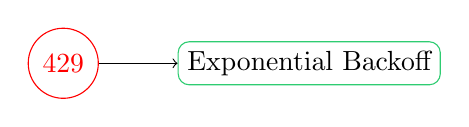
\begin{tikzpicture}
        \node (err) [draw=red, circle, text=red] {429};
        \node (wait) [right=of err, draw=Emerald, rounded corners] {Exponential Backoff};
        \draw[->] (err) -- (wait);
    \end{tikzpicture}
    \vfill
    \begin{itemize}
        \item \textbf{Wait Strategy}: Automatic cooldown (10s) between API hits.
        \item \textbf{Retry Logic}: Up to 5 retries with increasing delay.
        \item \textbf{Context Compression}: Truncating abstracts to save on Free-Tier TPM limits.
    \end{itemize}
\end{frame}

% --- Slide 13: The Q1 Pipeline Convergence ---
\begin{frame}{System Convergence}
    \centering
    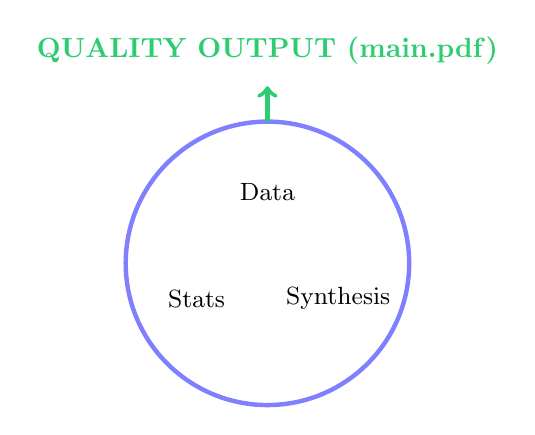
\begin{tikzpicture}[scale=0.9]
        \draw[ultra thick, blue!50] (0,0) circle (2cm);
        \node at (0,1) {\small Data};
        \node at (-1,-0.5) {\small Stats};
        \node at (1,-0.5) {\small Synthesis};
        \node at (0,3) [Emerald] {\textbf{QUALITY OUTPUT (main.pdf)}};
        \draw[->, ultra thick, Emerald] (0,2) -- (0,2.5);
    \end{tikzpicture}
\end{frame}

% --- Slide 14: Practical Case Study ---
\section{Results \& Impact}
\begin{frame}{Case Study: Decarbonization \& Equity}
    \begin{itemize}
        \item \textbf{Input}: Theme on intergenerational fiscal structures.
        \item \textbf{Process}: 25 Scopus papers retrieved, AI generated 5 thematic sections.
        \item \textbf{Output}: Comprehensive 12-page PDF with 35+ citations, fully compiled.
    \end{itemize}
\end{frame}

% --- Slide 15: System Limitations ---
\section{Critique \& Recommendations}
\begin{frame}{Current System Limitations}
    \begin{itemize}
        \item \textbf{API Dependency}: Tight coupling with Scopus and Gemini quotas.
        \item \textbf{Data Silo}: Currently restricted to a single bibliographic source (Scopus).
        \item \textbf{Linear Workflow}: Lack of "Human-in-the-loop" for real-time outline editing.
        \item \textbf{Computational Overhead}: R-Bibliometrix requires a full local R environment.
    \end{itemize}
\end{frame}

% --- Slide 16: Strategic Recommendations ---
\begin{frame}{Recommendations for Future Evolution}
    \begin{itemize}
        \item \textbf{Multi-DB Integration}: Expand to PubMed, CrossRef, and OpenAlex.
        \item \textbf{Hybrid LLM Core}: Use an ensemble of models (e.g., Gemini for speed, Claude for creative nuance).
        \item \textbf{Web Orchestrator}: Deploy as a FastAPI backend with a React/N8N visual frontend.
        \item \textbf{Zotero/Mendeley Bridge}: Automated export to reference management software.
    \end{itemize}
\end{frame}

% --- Slide 17: Future Roadmap ---
\begin{frame}{Future Horizons}
    \begin{itemize}
        \item \textbf{Knowledge Graphs}: Visualizing citation "trees" directly in LaTeX.
        \item \textbf{Real-time Synthesis}: Streaming generation of sections for interactive research.
    \end{itemize}
\end{frame}

% --- Slide 18: Conclusion ---
\begin{frame}{Conclusion}
    \centering
    \Large \textbf{Autonomous Research is No Longer Science Fiction.}
    \vfill
    \small 
    The ARA project demonstrates that by combining modular architecture, R-based analytics, and LLM-driven synthesis, we can accelerate scientific discovery by orders of magnitude.
    \vfill
    \textbf{Questions? Contact: Bilel Ammouri}
\end{frame}

\end{document}
